%%%%%%%%%%%%%%%%%%%%%%% file template.tex %%%%%%%%%%%%%%%%%%%%%%%%%
%
% This is a general template file for the LaTeX package SVJour3
% for Springer journals.          Springer Heidelberg 2010/09/16
%
% Copy it to a new file with a new name and use it as the basis
% for your article. Delete % signs as needed.
%
% This template includes a few options for different layouts and
% content for various journals. Please consult a previous issue of
% your journal as needed.
%
%%%%%%%%%%%%%%%%%%%%%%%%%%%%%%%%%%%%%%%%%%%%%%%%%%%%%%%%%%%%%%%%%%%
%
% First comes an example EPS file -- just ignore it and
% proceed on the \documentclass line
% your LaTeX will extract the file if required
\begin{filecontents*}{example.eps}
%!PS-Adobe-3.0 EPSF-3.0
%%BoundingBox: 19 19 221 221
%%CreationDate: Mon Sep 29 1997
%%Creator: programmed by hand (JK)
%%EndComments
gsave
newpath
  20 20 moveto
  20 220 lineto
  220 220 lineto
  220 20 lineto
closepath
2 setlinewidth
gsave
  .4 setgray fill
grestore
stroke
grestore
\end{filecontents*}
%
\RequirePackage{fix-cm}
%
%\documentclass{svjour3}                     % onecolumn (standard format)
%\documentclass[smallcondensed]{svjour3}     % onecolumn (ditto)
\documentclass[smallextended]{svjour3}       % onecolumn (second format)
%\documentclass[twocolumn]{svjour3}          % twocolumn
%
\smartqed  % flush right qed marks, e.g. at end of proof
%
\usepackage{amsmath}
\usepackage{xspace,stmaryrd,latexsym}
\usepackage{graphicx,tikz,rotating}
%
% \usepackage{mathptmx}      % use Times fonts if available on your TeX system
%
% insert here the call for the packages your document requires
%\usepackage{latexsym}
% etc.
%
% please place your own definitions here and don't use \def but
% \newcommand{}{}
%
% Insert the name of "your journal" with
% \journalname{myjournal}
%


\def\D{\mathbf{D}}
\def\E{\mathbf{E}}

\def\FFOL{\mathit{FFOL}}
\def\V{\mathit{V}}
\def\F{\mathit{F}}
\def\P{\mathit{P}}
\def\True{\mathit{True}}
\def\False{\mathit{False}}
\def\Impl{\rightarrow}
\def\Descr{\rotatebox[origin=C]{180}{$\iota$}}
%\def\Descr{\rotate[c]{180}{\iota}}


% -----------------------------------------------

\def\lambdot{\rule{0.6mm}{0.6mm}\hspace{0.4ex}} 
\def\all#1{\forall #1\lambdot}
\def\exi#1{\exists #1\lambdot}
\def\lam#1{\lambda #1\lambdot}


\def\modal#1{#1}
\def\mfalse{\modal\bot}
\def\mtrue{\modal\top}
\def\mnot{\modal\neg\,}
\def\mor{\,\modal\vee\,}
\def\mand{\,\modal\wedge\,}
\def\mimpl{\,\modal\supset\,}
\def\miff{\,\modal\Leftrightarrow\,}
\def\mball#1{\modal\Box_{#1}\,}
\def\mdexi#1{\modal\Diamond_{#1}\,}
\def\mall#1{\modal{\forall}{#1}\lambdot\,}
\def\mexi#1{\modal{\exists}{#1}\lambdot\,}
\def\mpi{\modal{\Pi}\,}
\def\mvalid{\modal{\texttt{valid}}} 

\def\Metaeq{=}
\def\bnormform#1{\left.#1\hspace*{-.4ex}\right\downarrow_\beta}
\def\benormform#1{\left.#1\hspace*{-.4ex}\right\downarrow_{\beta\eta}}
\def\Bnormform#1{\left.{#1}\hspace*{-.4ex}\right\downarrow_\beta}
\def\Benormform#1{\left.{#1}\hspace*{-.4ex}\right\downarrow_{\beta\eta}}
\def\ambnormform#1{{#1}\hspace*{-1.1ex}\downarrow_{\kern-.2em\scriptscriptstyle *}} % ``ambiguous'' normal form
\def\eqb{\Metaeq_{\beta}}
\def\eqe{\Metaeq_{\eta}}
\def\eqbe{\Metaeq_{\beta\eta}}
\def\convarrow{\rightarrow}


\newcommand\entity[1]{\text{\textrm{#1}}}
\def\QHL{\entity{QHL}}
\def\QML{\entity{QML}}
\def\NOM{\entity{NOM}}
\def\SVAR{\entity{SVAR}}
\def\CON{\entity{CON}}
\def\FVAR{\entity{FVAR}}
%\def\IC{\entity{IC}}
\def\FSYM{\entity{FSYM}}
\def\RSYM{\entity{RSYM}}
\def\QHLSTT{\entity{QHLSTT}}
\def\QMLSTT{\entity{QMLSTT}}
\def\IV{\entity{IV}}
\def\PV{\entity{PV}}
\def\SYM{\entity{SYM}}
\def\IVSTT{\entity{IVSTT}}
\def\PVSTT{\entity{PVSTT}}
\def\SYMSTT{\entity{SYMSTT}}
\def\SSTT{\entity{SSTT}}
\def\AR{\entity{AR}}
\def\STT{\entity{STT}\xspace}

\def\QKPIm{\entity{QK}\pi^-\xspace}
\def\QKPI{\entity{QK}\pi\xspace}
\def\QKPIp{\entity{QK}\pi^+\xspace}
\def\QSFPIm{\entity{QS5}\pi^-\xspace}
\def\QSFPI{\entity{QS5}\pi\xspace}
\def\QSFPIp{\entity{QS5}\pi^+\xspace}

\def\stt{\entity{STT}\xspace}
\def\tt{\entity{STT}}
\def\lm{\entity{MM}\xspace}
\def\ipl{\entity{IPL}\xspace}
\def\HOML{\entity{HOML}\xspace}
\def\HOL{\entity{HOL}\xspace}

\def\worldtype{\mu}
\def\indtype{\iota}
\def\mutype{\mu}
\def\boola{\omicron}
\def\boolb{\hat{\omicron}}

\def\ar{\shortrightarrow}

\newcommand\hol[1]{\boldsymbol{#1}}
\newcommand\lift[1]{\lceil #1 \rceil}
\newcommand\llift[1]{\dot{#1}}

\newcommand{\imp}{\supset}
\newcommand{\biimp}{\equiv}
\newcommand{\allq}{\forall}
\newcommand{\exq}{\exists}
\newcommand{\seq}{\vdash}
\newcommand{\nec}{\Box} % necessarily
\newcommand{\pos}{\Diamond} % possibly
\newcommand{\ess}[2]{#1 \ \mathit{ess.} \ #2}
\newcommand{\NE}{\mathit{NE}}


\begin{document}

\title{Exploring Axiom Systems for Category Theory%\thanks{Grants or other notes
%about the article that should go on the front page should be
%placed here. General acknowledgments should be placed at the end of the article.}
}
\subtitle{Utilizing a 
 Novel Approach to Automate Free Logic in HOL}

%\titlerunning{Short form of title}        % if too long for running head

\author{Christoph Benzm\"uller       \and
      Dana Scott 
}

%\authorrunning{Short form of author list} % if too long for running head

\institute{F. Author \at
              first address \\
              Tel.: +123-45-678910\\
              Fax: +123-45-678910\\
              \email{fauthor@example.com}           %  \\
%             \emph{Present address:} of F. Author  %  if needed
           \and
           S. Author \at
              second address
}

\date{Received: date / Accepted: date}
% The correct dates will be entered by the editor


\maketitle

\begin{abstract}
  % Partiality and undefinedness are prominent challenges in various
  % areas of mathematics and computer science.  Unfortunately, however,
  % modern proof assistant system based on traditional classical or
  % intuitionistic logics provide rather inadequate support for these
  % challenge concepts.  Free logic offers a theoretically appealing
  % solution, but is has been considered as rather unsuited towards
  % practical utilisation.

  % The two main contributions of this article are: (i) A shallow
  % semantical embedding of free logic in classical higher-order logic
  % is presented; this embedding enables the application of higher-order
  % interactive and automated theorem provers (and their integrated
  % subprovers) for the formalisation and verification of free logic
  % theories.  (ii) This approach to automate free logic is exemplarily
  % employed in a selected domain of mathematics: Starting from a
  % generalization of the standard axioms for a monoid we present a
  % stepwise development of various, mutually equivalent foundational
  % axiom systems for category theory. As a side-effect of this work
  % some (minor) issue in a prominent category theory textbook have been
  % revealed.

  A shallow semantical embedding of free logic in classical
  higher-order logic is presented, which enables the off-the-shelf
  application of higher-order interactive and automated theorem
  provers (and their integrated subprovers) for the formalisation and
  verification of free logic theories.  
  Subsequently, this approach is exemplarily employed in a selected domain of
  mathematics: starting from a generalization of the standard axioms
  for a monoid we present a stepwise development of various, mutually
  equivalent foundational axiom systems for category theory. As a
  side-effect of this work some (minor) issue in a prominent category
  theory textbook has been revealed.

The purpose of this article is not claim any novel results in category
theory, but to demonstrate an elegant way to ``implement'' and utilise
reasoning in free logic, and to present respective experiments.


\keywords{Free Logic \and Classical Higher-Order Logic \and Category
  Theory \and Interactive and Automated Theorem Proving }
% \PACS{PACS code1 \and PACS code2 \and more}
% \subclass{MSC code1 \and MSC code2 \and more}
\end{abstract}

\section{Introduction}
\label{intro}
Partiality and undefinedness are prominent challenges in various areas
of mathematics and computer science.  Unfortunately, however, modern
proof assistant systems and automated theorem provers based on
traditional classical or intuitionistic logics provide rather
inadequate support for these challenge concepts.  Free logic offers a
theoretically appealing solution, but is has been considered as rather
unsuited towards practical utilisation.


In the first part of this article (\S2 and \S3) we show how free logic
can be elegantly ``implemented'' in any theorem proving system for
classical higher-order logic (HOL) \cite{B5}. The proposed solution
employs a semantic embedding of free (or inclusive logic) in HOL. We
present an exemplary implementation of this idea in the mathematical
proof assistant Isabelle/HOL \cite{NPW02}. Various state-of-the-art
first-order and higher-order automated theorem provers and model
finders are integrated (modulo suitable logic translations) with
Isabelle via the Sledgehammer tool \cite{Sledgehammer}, so that our
solution can be utilized, via Isabelle as foreground system, with a
whole range of other background reasoners. As a result we obtain an
elegant and powerful implementation of an interactive and automated
theorem proving (and model finding) system for free logic.


%   The two main contributions of this article are: (i) A shallow
%   semantical embedding of free logic in classical higher-order logic
%   is presented; this embedding enables the application of higher-order
%   interactive and automated theorem provers (and their integrated
%   subprovers) for the formalisation and verification of free logic
%   theories.  (ii) This approach to automate free logic is exemplarily
%   employed in a selected domain of mathematics: Starting from a
%   generalization of the standard axioms for a monoid we present a
%   stepwise development of various, mutually equivalent foundational
%   axiom systems for category theory. As a side-effect of this work
%   some (minor) issue in a prominent category theory textbook have been
%   revealed.



% Partiality and undefinedness are core concepts in various areas of
% mathematics.  Modern mathematical proof assistants and theorem proving
% systems are often based on traditional classical or intuitionistic
% logics and provide rather inadequate support for these challenge
% concepts.  Free logic @{cite "sep-logic-free,scott67:exist"}, in
% contrast, offers a theoretically and practically appealing
% solution. Unfortunately, however, we are not aware of any implemented
% and available theorem proving system for free logic.
 
% In this extended abstract we show how free logic can be
% ``implemented'' in any theorem proving system for classical
% higher-order logic (HOL) @{cite "B5"}. The proposed solution employs a
% semantic embedding of free (or inclusive logic) in HOL. We present an
% exemplary implementation of this idea in the mathematical proof
% assistant Isabelle/HOL @{cite "NPW02"}. Various state-of-the-art
% first-order and higher-order automated theorem provers and model
% finders are integrated (modulo suitable logic translations) with
% Isabelle via the Sledgehammer tool @{cite "Sledgehammer"}, so that our
% solution can be utilized, via Isabelle as foreground system, with a
% whole range of other background reasoners. As a result we obtain an
% elegant and powerful implementation of an interactive and automated
% theorem proving (and model finding) system for free logic.
  
To demonstrate the practical relevance of our new system, we present,
in the second part of this article, a stepwise development of axiom
systems for category theory by generalizing the standard axioms for a
monoid to a partial composition operation. Our purpose is not to make
or claim any contribution to category theory but rather to show how
formalizations involving the kind of logic required (free logic) can
be validated within modern proof assistants.

A total of eight different axiom systems is studied. The systems I-VI
are shown to be equivalent. The axiom system VII slightly modifies
axiom system VI to obtain (modulo notational transformation) the set
of axioms as proposed by Freyd and Scedrov in their textbook
``Categories, Allegories'' \cite{FreydScedrov90}, published in 1990;
see also Subsection \ref{subsec:FreydNotation} where we present their
original system.  While the axiom systems I-VI are shown to be
consistent, a constricted inconsistency result is obtained for system
VII (when encoded in free logic where free variables range over all
objects): We can prove $\exists x. \neg(E x) \Impl False$, where
$E$ is the existence predicate. Read this as: If there are undefined
objects, e.g. the value of an undefined composition $x\cdot y$
then we have falsity.  By contraposition, all objects (and thus all
compositions) must exist. But when we assume the latter, then the
axiom system VII essentially reduces categories to monoids.  We note
that axiom system V, which avoids this problem, corresponds to a set
of axioms proposed by Scott @{cite "Scott79"} in the 1970s. The
problem can also be avoided by restricting the variables in axiom
system VII to range only over existing objects and by postulating
strictness conditions.  This gives us axiom system VIII.

Our exploration has been significantly supported by series of experiments in which automated reasoning tools 
have been called from within the proof assistant Isabelle/HOL @{cite "Isabelle"} via the Sledgehammer 
tool @{cite "Sledgehammer"}. Moreover, we have obtained very useful feedback at various stages 
from the model finder Nitpick @{cite "Nitpick"} saving us from making several mistakes.

At the conceptual level this paper exemplifies a new style of explorative mathematics which rests 
on a significant amount of human-machine interaction with integrated interactive-auto\-ma\-ted 
theorem proving technology. The experiments we have conducted are such that the required 
reasoning is often too tedious and time-consuming for humans to be carried out repeatedly with 
highest level of precision. It is here where cycles of formalization and experimentation efforts in 
Isabelle/HOL provided  significant support. Moreover, the technical inconsistency issue for
axiom system VII was discovered by automated theorem provers, which further emphasises the added 
value of automated theorem proving in this area. 

The content of article is combines, extends and clarifies the
contributions reported in two previous papers \cite{ICMS,ArXiv}.

% To enable our experiments we have exploited an embedding of free logic @{cite "Scott67"} 
% in classical higher-order logic, which we have recently presented in a related paper @{cite "C57"}.


% We also want to emphasize that this paper has been written entirely within the Isabelle 
% framework by utilizing the Isabelle ``build'' tool; cf. @{cite "IsabelleManual2016"}, Section~2. 
% It is thus an example of a formally verified mathematical document, where the PDF document as 
% presented here has been generated directly from the verified source files mentioned above.
% We also note that once the proofs have been mechanically checked, they are generally easy 
% to find by hand using paper and pencil.

\section{Preliminaries}
\label{sec:preliminaries}
\subsection{Free Logic}
Free logic \cite{Lambert60,Scottt} refers to a class of logic
formalisms that are free of basic existence assumptions regarding the
denotation of terms. Remember that terms in e.g. traditional classical
and intuitionistic predicate logics always denote an (existing) object
in a given (non-empty) domain $\D$, and that $\D$ is also exactly the set the
quantifiers range over. In free logic these
basic assumption are abolished. Terms do still denote objects in a
(non-empty) domain $\D$, but a (possibly empty) set $\E\subseteq \D$ is
chosen to characterize the subdomain of ``existing'' resp. ``defined''
objects in $\D$. Quantification is
now restricted to set $\E$ of existing/defined objects only. It is
obvious how this can be used to model undefideness and partiality:
problematic terms, e.g. division by zero or improper definite
descriptions, still denote, but they refer to undefined objects, that
is, objects $d$ in $\D\setminus \E$ lying outside of the scope of
quantification.  

The particular notion of free logic as exploited in the remainder of
this article has been introduced by Scott \cite{Scott67}.  A graphical
illustration of this notion of free logic is presented in
Fig.~\ref{fig1}. It
employs a distinguished undefined object $\star$.  
% Free logic (and inclusive logic) has been proposed as an alternative
% to remedy these shortcomings. It distinguishes between a raw domain of
% possibly non-existing objects ‹❙D› and a particular subdomain ‹❙E› of ‹❙D›,
% containing only the ``existing'' entities. Free variables range over ‹❙D›
% and quantified variables only over ‹❙E›. Each term denotes in ‹❙D› but not
% necessarily in ‹❙E›. The particular notion of free logic as exploited below has been
% introduced by Scott @{cite "scott67:_exist"}. A graphical 
% illustration of this notion of free logic is presented in Fig.~\ref{fig1}.
\begin{figure}
\centering
\newcommand\firstellipse{(2,-5) ellipse (6cm and 4cm)}
\newcommand\secondellipse{(0,-5.3) ellipse (3.5cm and 2.5cm)}1
\begin{tikzpicture}
  \begin{scope}[fill opacity=1]
    \fill[gray!40] \firstellipse;
    \fill[gray!10] \secondellipse;
  \end{scope}
  \begin{scope}[very thick,font=\large]
    \draw \firstellipse node[font=\normalsize\bfseries] at (-.5,-5) {\underline{\textbf{E}: existing objects}};
    \draw \firstellipse node[font=\small] at (-.5,-5.5) {values of bound variables};
    \draw \secondellipse node[font=\normalsize\bfseries] at (4.3,-2.5) {\underline{\textbf{D}: raw objects}};
    \draw \secondellipse node[font=\small] at (4.3,-3) {values of free variables};
  \end{scope}
  \node[font=\normalsize\bfseries] at (6,-5) {$\star$};
  \node[font=\normalsize\bfseries] at (6,-5.3) {undefined};
\end{tikzpicture}
\caption{Illustration of the Semantical Domains of Free Logic \label{fig1}}
\end{figure}

We now formally introduce the syntax and semantics of free logic as
assumed in the remainder of this article. We refer to this logic with $\FFOL$.

\begin{definition}[Syntax of $\FFOL$]
  We start with a denumerable set $\V$ of variable symbols, a denumerable set
  $\F$ of $n$-ary function symbols ($n\geq 0$), and a denumerable set
  $\P$ of $n$-ary predicate symbols ($n\geq 0$).

  The terms and formulas of $\FFOL$ are formally defined as the
  smallest sets such that:
\begin{enumerate}
\item each variable $x\in\V$ is a term of $\FFOL$, 
\item given any $n$-ary ($n\geq 0$) function symbol $f\in\F$ and terms
  $t_1,\ldots,t_n$ of $\FFOL$, then $f(t_1,\ldots,t_n)$ is a term of $\FFOL$, 
\item given terms $t_1$ and $t_2$ of $\FFOL$, then $t_1 = t_2$ is an
  (atomic) formula of $\FFOL$,
\item given any $n$-ary ($n\geq 0$) predicate symbol $p\in\P$ and terms
$t_1,\ldots,t_n$ of $\FFOL$, then $p(t_1,\ldots,t_n)$ is an (atomic)
formula of $\FFOL$, 
\item given formulas $r$ and $s$ of $\FFOL$, then $\neg r$, $r
  \Impl s$ and $\forall x. r$ are (compound) formulas of $\FFOL$
\item given a formula $r$ of $\FFOL$, then $\Descr x. r$ is a
  term of $\FFOL$ (definite  description)
\end{enumerate}
\end{definition}

Further formulas of $\FFOL$  can be defined as usual.

Regarding the semantics different options may be considered. For
example, instead of a possible empty set of existing objects $E$, we
could postulate non-emptiness of $E$. We e.g. also have a choice when
interpreting equations $t = t$ for undefined terms $t$; such equations
could be mapped to $\True$ or $\False$. Different combinations of such
choice points have been studied in the literature. Here we closely
follow the logic of Scott \cite{Scott67}.

\begin{definition}[Dual-domain (positive) semantics of $\FFOL$]
  A model structure for $\FFOL$ consists of a triple
  $\langle D, E, I, \star\rangle$, where $D$ is a non-empty raw domain of
  objects, $E\subseteq D$ a possible empty set of ``existing''
  resp. ``defined'' objects, and $I$ an interpretation function
  mapping 0-ary function symbols (constants) to defined objects $d\in E$, 
 0-ary predicate symbols (propositions) to $\True$ or $\False$, 
  $n$-ary function symbols (for $n\geq 1$) to $n$-ary functions
  $D \times \ldots \times D \longrightarrow D$ and $n$-ary predicate
  symbols (for $n\geq 1$) to $n$-ary relations
  $D \times \ldots \times D$. Finally, $\star\in D\setminus E$ is a designated
  (non-existing/undefined) object. 

  Given a variable assignment $g: \V \longrightarrow D$, we
  define the interpretation function $\|\cdot\|^{I,g}$ for terms and formulas of
  $\FFOL$ as follows:
\noindent
\begin{description}
\item{Terms}
\begin{enumerate}
\item $\| x \|^{I,g} = g(x)$ for variable symbols $x\in\F$
\item $\| c \|^{I,g} = I(c)$, where $c\in\F$ is an 0-ary function symbol
\item $\| f(t_1,\ldots,t_n)\|^{I,g} = I(f)(\| t_1 \|^{I,g},\ldots,\|
  t_n \|^{I,g})$, where $f\in\F$ is an $n$-ary ($n\geq 1$) function symbol
\item $\| \Descr x. r \|^{I,g} = d \in E$, such that $\| r
  \|^{I,g[d/x]} = \True$ and  $\| r
  \|^{I,g[d'/x]} = \False$ for all $d'\not=d\in E$ (i.e. $d$ is the
  unique existing object for which $r$ holds); if there is no
  such $d\in E$, then $\| \Descr x. r \|^{I,g} = \star$
\end{enumerate}

\item{Formulas}
\begin{enumerate}
\item $\| p \|^{I,g} = I(p)$, where $p\in\F$ is an 0-ary predicate
  symbol
\item $\| t_1 = t_2 \|^{I,g} = \True$ iff $\| t_1 \|^{I,g} = \| t_2
  \|^{I,g}$ (this implies that equations such as $1/0 = 1/0$ are
  evaluated to $\True$; however, we have alternative options do define
  this case: e.g. we could
  additionally require that $\| t_1 \|^{I,g} \in E$ and
  $\| t_2 \|^{I,g} \in E$, in which case $1/0 = 1/0$ would be $\False$).
\item $\| p(t_1,\ldots,t_n) \|^{I,g} = \True$ iff $(\| t_1 \|^{I,g},\ldots,\|
  t_n \|^{I,g}) \in I(p)$ for $n$-ary ($n\geq 1$) predicate symbols
  $p\in\P$
\item $\| \neg r \|^{I,g} = \True$ iff $\| r \|^{I,g} = \False$
\item $\| r \Impl s \|^{I,g} = \True$ iff $\| r \|^{I,g} = \False$
  or $\| s \|^{I,g} = \True$
\item $\| \forall x. r  \|^{I,g} = \True$ iff for all $d \in E$ we
  have $\|  r  \|^{I,g[d/x]} = \True$ (here $g[d/x]$ denotes the
  variable assignment that is identical to $g$, except for variable
  $x$, which is now mapped to object $d$)
\end{enumerate}
\end{description}

\end{definition}
 

\begin{definition}\label{homlvalid}
  A formula $s_o$ is \emph{true} in model $M$ under assignment $g$ iff
  $\|s_o\|^{M,g} = T$; this is also denoted as $M,g \models s_o$.  A
  formula $s_o$ is called \emph{valid} in $M$, which is denoted as
  $M \models s_o$, iff $M,g \models s_o$ for all assignments
  $g$. Finally, a formula $s_o$ is called \emph{valid}, which we
  denote by $\models s_o$, iff $s_o$ is valid for all $M$. Moreover,
  we write $\Gamma\models \Delta$ (for sets of formulas $\Gamma$ and
  $\Delta$) iff there is a model $M$ and an assignment $g$ such that
  $M,g \models s_o$ for all $s_o\in \Gamma$ and $M,g \models t_o$ for
  at least one $t_o\in \Delta$.
\end{definition}


\subsection{Classical higher-order logic}
\HOL is easily obtained from \HOML by removing the modal operator
$\Box$ from the grammar, and by dropping the set of possible worlds
$W$ and the accessibility relation $R$ from the definition of a model.
Nevertheless, we explicitly state the most relevant definitions for
the particular notion of \HOL as employed in this paper. One reason is
that we do want to carefully distinguish the \HOL and \HOML languages
in the remainder (we use boldface fonts for \HOL and standard fonts
for \HOML). There is also a subtle, but harmless, difference in the
\HOL language as employed here  in comparison to the standard
presentation: here three base types are employed, whereas
usually only two base types are considered. The third base type plays
a crucial role in our embedding of \HOML in \HOL.


\begin{definition}\label{holtypes}
  The set $\hol{T}$ of simple types freely generated from a set of
  basic types $\{\hol{o}, \hol{\mu}, \hol{\iota}\}$ using the function type
  constructor $\hol{\ar}$. $\hol{o}$ is the type of Booleans,
  $\hol{\mu}$ is the type of individuals, and type
  $\hol{\iota}$ is employed as the type of possible worlds below. As
  before we may avoid parentheses.
\end{definition}

\begin{definition}\label{holgrammar}
The grammar for higher-order logic $\HOL$ is:
\begin{align*} 
  \hol{s},\hol{t} \quad ::= \quad & \hol{p_\alpha} \mid \hol{X_\alpha} \mid \hol{(\lam{X_\alpha}
  s_\beta)_{\alpha\ar\beta}} \mid \hol{(s_{\alpha\ar\beta}\, t_\alpha)_\beta} \mid  \hol{\neg_{o\ar o}\, s_o} \mid \\
  & \hol{(({\vee_{o\ar o\ar o}}\,s_o)\,t_o)} \mid \hol{\forall_{(\alpha\ar
    o)\ar o}(\lam{X_\alpha} s_o)} 
\end{align*}
where $\hol{\alpha},\hol{\beta}\in \hol{T}$. The text from
Def.~\ref{homlgrammar} analogously applies, except that we do not
consider the modal  connectives $\hol{\Box}$ and $\hol{\Diamond}$.
\end{definition}

The definitions for substitution (Def.~\ref{homlsubstitution}), $\beta$- and $\eta$-reduction (Def.~\ref{homlbetaeta}), frame (Def.~\ref{homlframe}), and assignment (Def.~\ref{homlassignment}) remain unchanged.

\begin{definition}\label{holmodel}
  A \emph{model} for \HOL is a tuple $\hol{M}=\hol{\langle D, I \rangle}$, where
  $\hol{D}$ is a frame, and $\hol{I}$ is a family of typed interpretation
  functions mapping constant symbols $\hol{p_\alpha}$ to appropriate
  elements of $\hol{D_\alpha}$, called the \emph{denotation of $\hol{p_\alpha}$}
  (the logical connectives $\hol{\neg}$, $\hol{\vee}$, and $\hol{\forall}$ are always
  given the standard denotations, see below).  Moreover, we assume that the domains
  $\hol{D_{\alpha\ar\alpha\ar o}}$ contain the respective identity relations.
\end{definition}


\begin{definition}\label{holvalue}
  The \emph{value} $\hol{\| s_\alpha\|^{M,g}}$ of a \HOL term
  $\hol{s_\alpha}$ on a model $\hol{M}=\hol{\langle D, I \rangle}$ under assignment $\hol{g}$ is an element $\hol{d}\in \hol{D_\alpha}$
  defined in the following way:
\begin{enumerate}
\item $\hol{\|p_\alpha\|^{M,g}} = \hol{I(p_\alpha)}$ and $\hol{\|X_\alpha\|^{M,g}} = \hol{g(X_\alpha)}$
\item $\hol{\|(s_{\alpha\ar\beta}\, t_\alpha)_\beta\|^{M,g}} = \hol{\|s_{\alpha\ar\beta}\|^{M,g}(\|t_\alpha\|^{M,g})}$
\item $\hol{\|(\lam{X_\alpha}s_\beta)_{\alpha\ar\beta}\|^{M,g}} = $
  the function $\hol{f}$ from $\hol{D_\alpha}$ to $\hol{D_\beta}$ such
  that $\hol{f(d)} = \hol{\|s_\beta\|^{M,g[d/X_\alpha]}}$ for all
  $\hol{d}\in \hol{D_\alpha}$
\item $\hol{\|(\neg_{o\ar o}\, s_o)_o\|^{M,g}} = \hol{T}$ iff $\hol{\|s_o\|^{M,g}} = \hol{F}$
\item $\hol{\|(({\vee_{o\ar o\ar o}}\,s_o)\,t_o)_o\|^{M,g}} =
  \hol{T}$ iff\, $\hol{\|s_o\|^{M,g}} = \hol{T}$ or $\hol{\|t_o\|^{M,g}}
  = \hol{T}$
\item $\hol{\|(\forall_{(\alpha\ar o)\ar o}(\lam{X_\alpha}
    s_o))_o\|^{M,g}} = \hol{T}$ iff for all $\hol{d}\in
  \hol{D_\alpha}$ we have $\hol{\|s_o\|^{M,g[d/X_\alpha]}} = \hol{T}$
%\item $\|(\Box_{o\ar o}\, s_o)_o\|^{M,g,w} = T$ iff for all $v \in W$ with $w R v$ we have  $\|s_o\|^{M,g,v}  = T$
\end{enumerate}
\end{definition}


\begin{definition}\label{homlhenkinmodel}
 A model $\hol{M}=\hol{\langle D, I \rangle}$ is called a
 \emph{standard model} iff for all $\alpha,\beta\in T$ we have
 $D_{\alpha\ar\beta} = \{ f \mid f : D_\alpha \longrightarrow D_\beta
 \}$. In a \emph{Henkin model} function spaces are not necessarily
 full. Instead it is only required that $D_{\alpha\ar\beta}
 \subseteq \{ f \mid f : D_\alpha \longrightarrow D_\beta \}$ (for all
 $\alpha,\beta\in T$) and that the valuation function 
 $\|\cdot\|^{M,g}$ from above is total (i.e., every term denotes). Any standard model is obviously
 also a Henkin model. We consider Henkin models in the remainder.
\end{definition}

\begin{definition}\label{homlvalid}
A formula $s_o$ is \emph{true} in model $M$ 
under assignment $g$ iff $\|s_o\|^{M,g} = T$; this is also denoted
as $M,g \models s_o$.  A formula $s_o$ is called \emph{valid} in
$M$, which is denoted as $M \models s_o$, iff $M,g \models s_o$ for all
assignments $g$. Finally, a formula $s_o$ is called
\emph{valid}, which we denote by $\models s_o$, iff $s_o$ is valid for
all $M$. Moreover, we write $\Gamma\models \Delta$ (for sets of
 formulas $\Gamma$ and $\Delta$) iff there is a model $M$ and an assignment $g$ such that  
 $M,g \models s_o$ for all $s_o\in \Gamma$ and $M,g \models t_o$ for at least one $t_o\in \Delta$.
\end{definition}

% The definition for standard and Henkin models
% (Def.~\ref{homlhenkinmodel}), and for truth in a model, validity,
% etc. (Def.~\ref{homlvalid}) are adapted in the obvious way, and we use
% the notation $\hol{M,g \models s_o}$, $\hol{\models s_o}$, and
% $\hol{\Gamma \models \Delta}$. As for \HOML, we assume Henkin
% semantics in the remainder.



\section{Sound and Complete Embedding in HOL}
Todo ... the embedding in Isabelle/HOL is depicted in 
figure \ref{pic1}

\begin{figure}[t]
 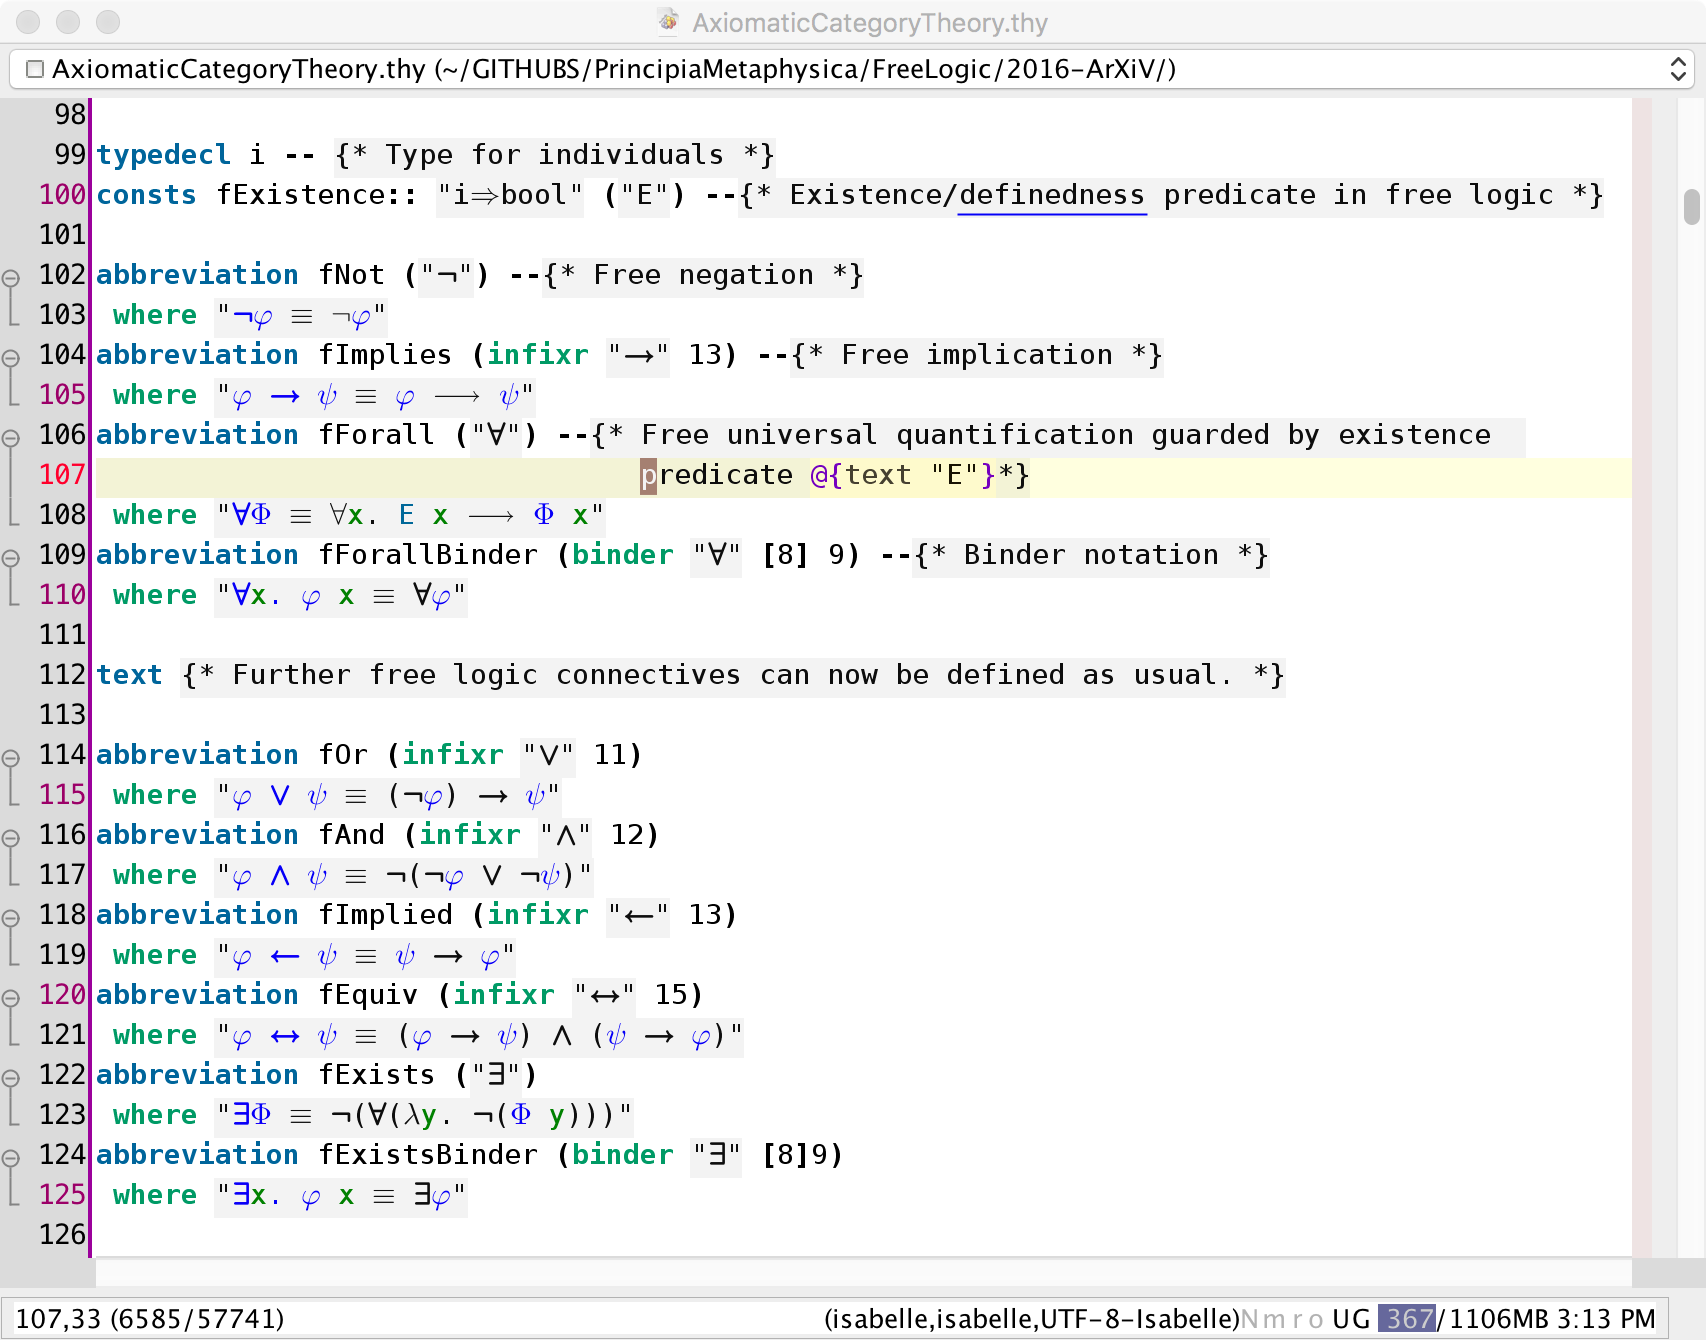
\includegraphics[width=\textwidth]{EmbeddingPic}
 \caption{Isabelle/HOL formalisation of $\FFOL$ in $\HOL$ \label{pic1}}
\end{figure}


\pagebreak
\newpage

\section{Section title}
\label{sec:1}
Text with citations \cite{RefB} and \cite{RefJ}.
\subsection{Subsection title}
\label{sec:2}
as required. Don't forget to give each section
and subsection a unique label (see Sect.~\ref{sec:1}).
\paragraph{Paragraph headings} Use paragraph headings as needed.
\begin{equation}
a^2+b^2=c^2
\end{equation}

% For one-column wide figures use
\begin{figure}
% Use the relevant command to insert your figure file.
% For example, with the graphicx package use
  
\includegraphics{example.eps}
% figure caption is below the figure
\caption{Please write your figure caption here}
\label{fig:1}       % Give a unique label
\end{figure}
%
% For two-column wide figures use
\begin{figure*}
% Use the relevant command to insert your figure file.
% For example, with the graphicx package use
  
\includegraphics[width=0.75\textwidth]{example.eps}
% figure caption is below the figure
\caption{Please write your figure caption here}
\label{fig:2}       % Give a unique label
\end{figure*}
%
% For tables use
\begin{table}
% table caption is above the table
\caption{Please write your table caption here}
\label{tab:1}       % Give a unique label
% For LaTeX tables use
\begin{tabular}{lll}
\hline\noalign{\smallskip}
first & second & third  \\
\noalign{\smallskip}\hline\noalign{\smallskip}
number & number & number \\
number & number & number \\
\noalign{\smallskip}\hline
\end{tabular}
\end{table}


%\begin{acknowledgements}
%If you'd like to thank anyone, place your comments here
%and remove the percent signs.
%\end{acknowledgements}

% BibTeX users please use one of
%\bibliographystyle{spbasic}      % basic style, author-year citations
\bibliographystyle{spmpsci}      % mathematics and physical sciences
%\bibliographystyle{spphys}       % APS-like style for physics
\bibliography{bibliography}   % name your BibTeX data base

% % Non-BibTeX users please use
% \begin{thebibliography}{}
% %
% % and use \bibitem to create references. Consult the Instructions
% % for authors for reference list style.
% %
% \bibitem{RefJ}
% % Format for Journal Reference
% Author, Article title, Journal, Volume, page numbers (year)
% % Format for books
% \bibitem{RefB}
% Author, Book title, page numbers. Publisher, place (year)
% % etc
% \end{thebibliography}

\end{document}
% end of file template.tex

